\documentclass[ignorenonframetext,10pt]{beamer}
%\documentclass[paper=a4,12pt,version=last,landscape]{scrartcl}

%\usepackage[latin1]{inputenc}
\usepackage[english]{babel}
\usepackage{amsmath,amssymb}
\usepackage{multimedia}
\usepackage{alltt}
\usepackage{multirow}
\usepackage{textcomp}
\usepackage[footnotesize]{subfigure}
\usepackage{graphicx}


\usepackage{pgfplots}
\pgfplotsset{width=7cm,compat=1.3}% <-- moves axis labels near ticklabels (respects tick label widths)
\usepackage{pgfplotstable}



%\usetheme{Berlin}
\usetheme{Darmstadt}
\useoutertheme[subsection=false]{miniframes}
\useoutertheme{smoothbars}
\usefonttheme{structurebold}
%\setbeamertemplate{navigation symbols}{}
\setbeamercovered{invisible}


\title{Helices indices of RNAs}
\author{\large Jiabin~Huang}
\date{\today}

\institute[ExpBI]{\normalsize
  AG Experimentelle Bioinformatik (Cyanolab)\\
  Institut f\"ur Biologie III\\
  Universit\"at Freiburg}
\subject{Talk based on Giegerich, Voss, Rehmsmeier (2004) ''Abstract
Shapes of RNA'' Nucleic Acids Research Vol. 32 No. 16}
  
  


\begin{document}

\frame{\maketitle}

% frame 2
\begin{frame}
\frametitle{Outline}
   \begin{itemize}
   \item an overview of RNA secondary structure elements and a classical RNA secondary structure prediction algorithm
   \item introducing concept of abstract shapes  
   \item basic idea about the helices indices
   \item outlook            
   \end{itemize}
\end{frame}


% PART 1: RNA secondary structure elements and Zuker algorithm
% frame 3  
\begin{frame}
\frametitle{Secondary structure elements of RNA}  
\begin{figure}
  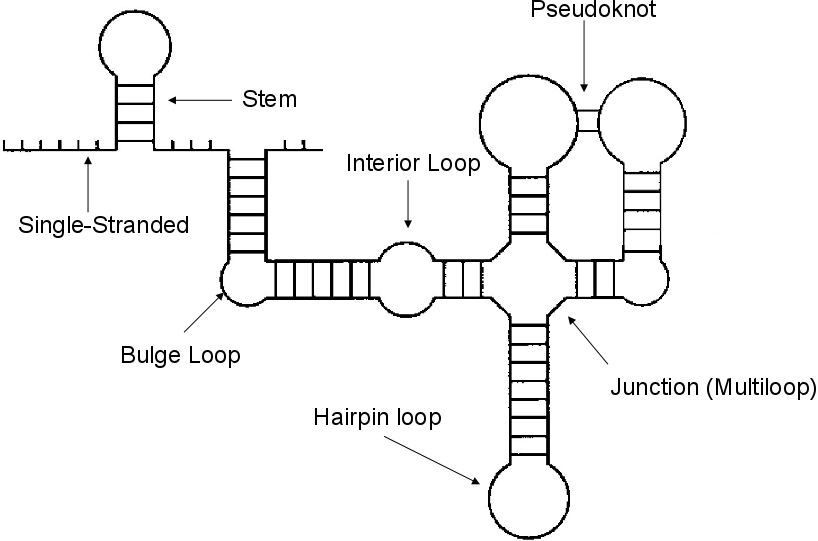
\includegraphics[scale=0.38]{images/RNA_components.jpg} 
  \caption{Structural elements}
\end{figure}
\end{frame}


% frame 4
\section{RNA folding by free energy minimization}
\subsection{}
\begin{frame}
\frametitle{\large Classical secondary structure algorithms (Zuker 1981)}
  \begin{block}{facts about Zuker algorithm}
    \begin{itemize}
    \item first described by Zuker and Stiegler in 1981
    \item assumption: There are no knots (base pairs never cross).
    \item basic idea: 
    \begin{enumerate}
      \item a RNA sequence can be folded into many different secondary structure
      \item for every secondary structure, we can calculate a free energy value
      \item after that, the algorithm choose the structure with the minimum free energy
    \end{enumerate}
    \item the runtime is $O(n^3)$
    \item can get only one solution
    \end{itemize}
  \end{block}
\end{frame}


% frame 5
\begin{frame}
\frametitle{Free energy computation example}  
\begin{figure}
  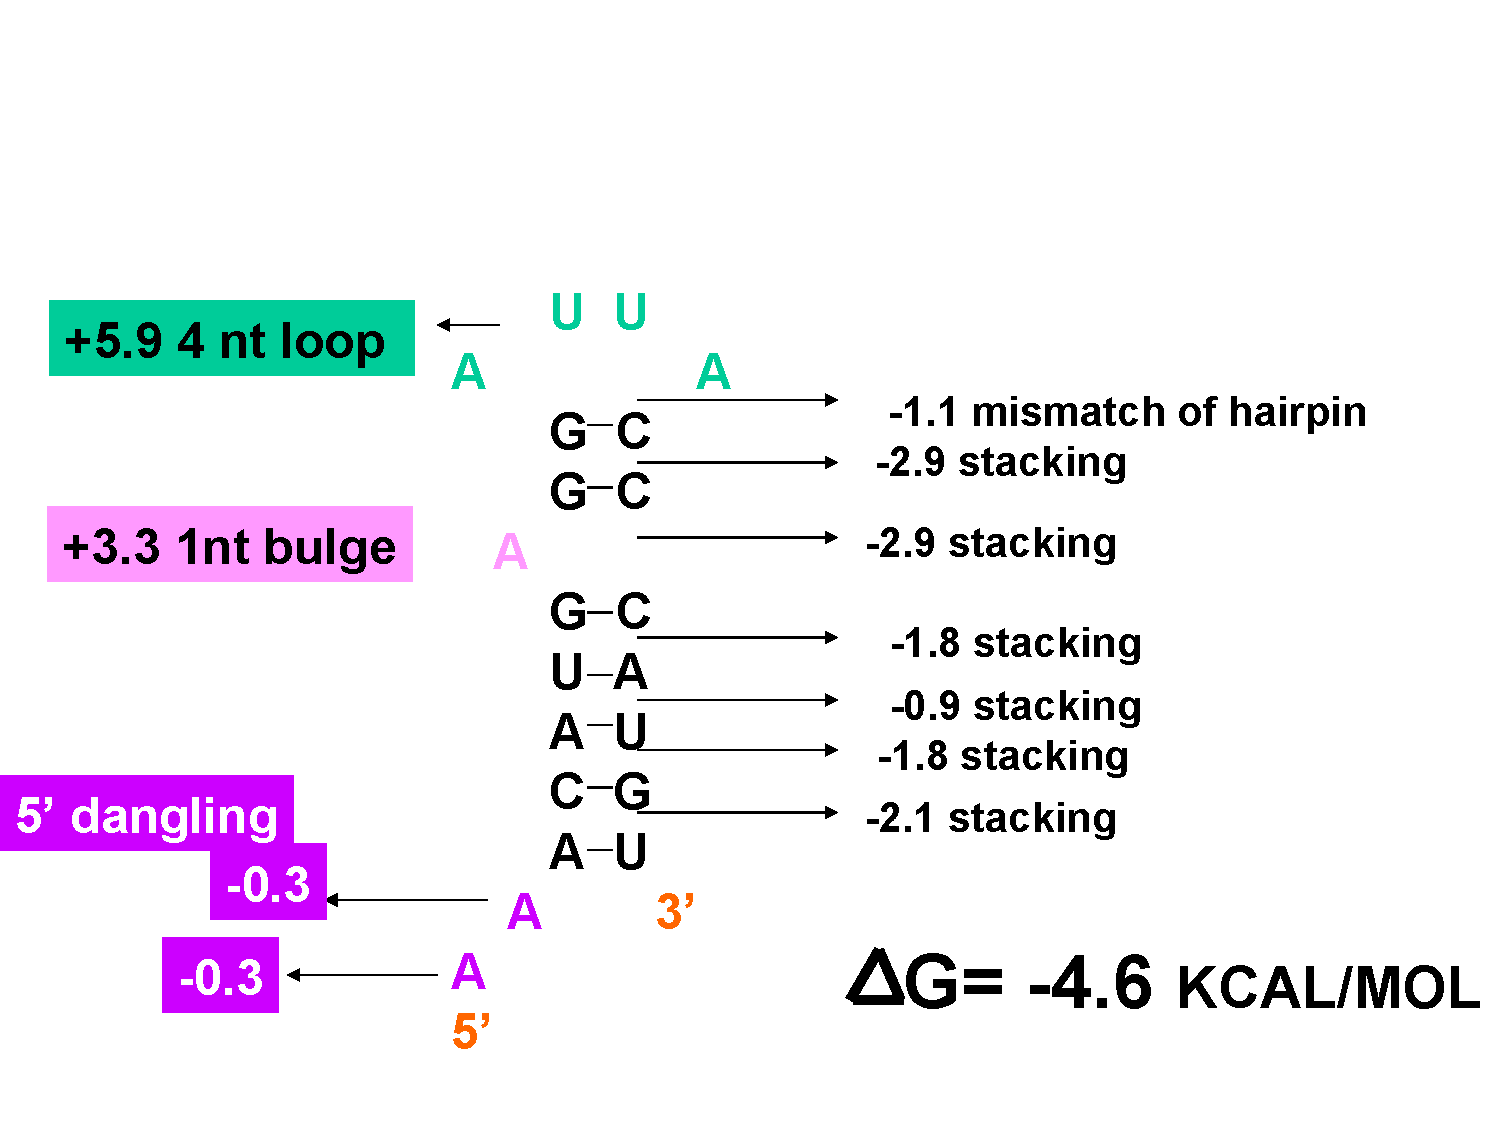
\includegraphics[scale=0.4]{images/mfe_example.pdf} 
\end{figure}
\end{frame}


% frame 6
\begin{frame}
\frametitle{energy landscape}
\begin{figure}
  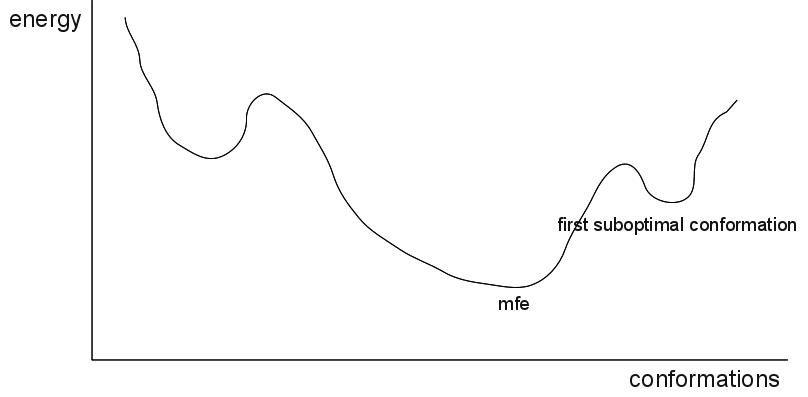
\includegraphics[scale=0.4]{images/energy_landscape_simple.jpg}
\end{figure}
\end{frame}


% frame 7  
\begin{frame}
\frametitle{Suboptimal structures}
  %\begin{block}
  \begin{itemize} 
    \item but the ''true'' structure is not always the one with the lowest predicted free energy.
    \item but it is not far away from the mfe and it is normally a local minimum
    \item one of solution: enumerate all suboptimal structures within a given energy range
    \item but the number of suboptimal structures grows exponentially with the energy range considered.
  \end{itemize}
  %\end{block}   
\end{frame}


% frame 8
\begin{frame}
\frametitle{energy landscape setting a range}  
\begin{figure}
  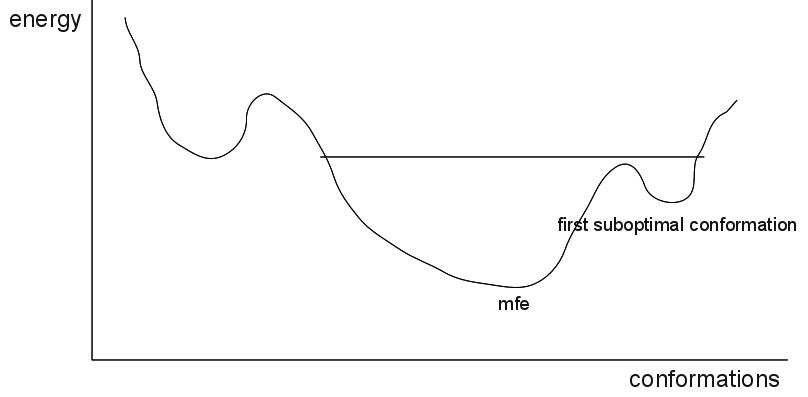
\includegraphics[scale=0.4]{images/energy_landscape_area.jpg} 
\end{figure}
\end{frame}


% PART 2: abstract shapes
% frame 9
\begin{frame}
\frametitle{Introducing abstract shapes}
    Solution: Use abstract shapes to describe a set of structures.
    \begin{itemize} 
    \item developed by Giegerich and Voss
    \item An abstract shape represents a class of similar structures sharing a
    common pattern of helix nesting and adjacency.
    \item ''Abstract'' since we do not care about all details of the structures.
    \item Each shape class has a representative structure called shrep (with minimum folding energy).
    \end{itemize}
\end{frame}


% frame 10
\begin{frame}
\frametitle{Abstract shape, energy range: 5 kcal/mol}  
\begin{figure}
  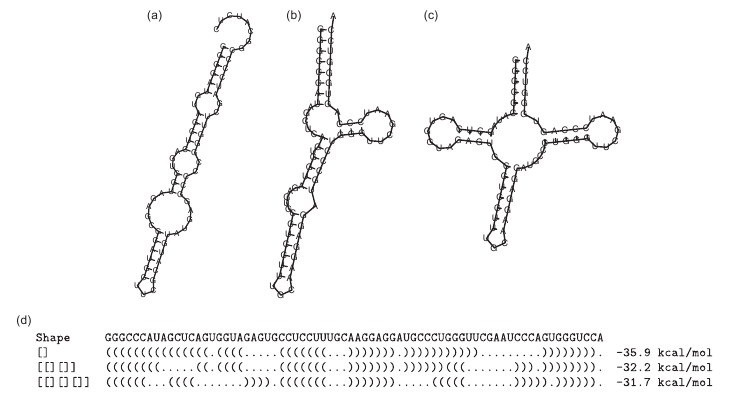
\includegraphics[scale=0.6]{images/shapes_example.jpg} 
\end{figure}
\end{frame}


% PART 3: helices indices
% frame 11
\section{develop a new structure abstraction}
\frametitle{Drawback of abstract shape}
\subsection{}
\begin{frame}
\frametitle{}
   \begin{block}{\small Drawback of abstract shape}
   \begin{itemize} 
   \item The major drawback of abstract shape analysis is the position
   independence of the abstraction
   \end{itemize}
   \end{block}
   \begin{block}{\small Drawback example 1 of abstract shape}
   \begin{figure}
     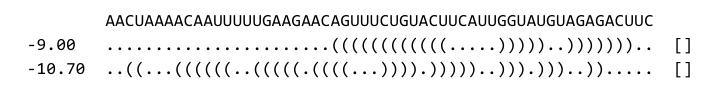
\includegraphics[scale=0.55]{images/drawback_1.jpg} 
   \end{figure}
   \end{block}
   \begin{block}{\small Drawback example 2 of abstract shape}
   \begin{figure}
     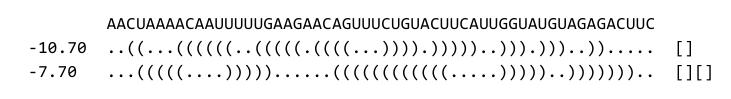
\includegraphics[scale=0.55]{images/drawback_2.jpg} 
   \end{figure}
   \end{block}
\end{frame}


% frame 12
\begin{frame}
\frametitle{develop a new structure abstraction}
    The straightforward idea to overcome the position independence of the
    current available shape abstractions is
    \begin{block}{the position of which secondary structure elements will be
    tracked}
    \begin{itemize} 
    \item helical regions of hairpin loop
    \item helical regions of multiloops %, as possible braching points, are structurally important    
    \item helical regions of stacked pairs, bulge and internal loops %are the main structural contributors 
    \end{itemize}
    \end{block}
    \begin{block}{which positions of the vordefined structure element will be tracked}
    \begin{itemize} 
    \item i
    \item j   
    \item (i,j)
    \item i+j/2
    \end{itemize}    
    \end{block}
\end{frame}

% frame 13
% frame landscape
\begin{frame}
\frametitle{helices positions example}  
\begin{figure}
  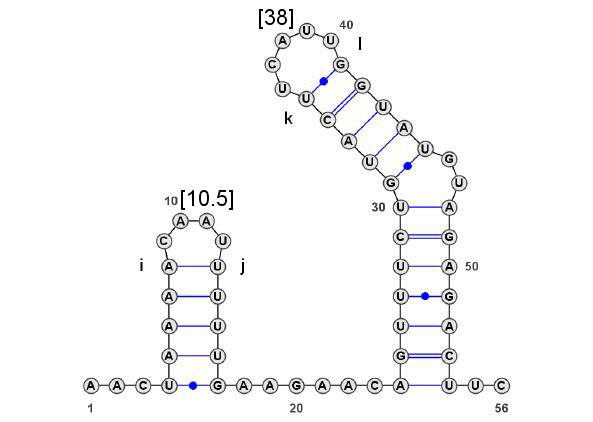
\includegraphics[scale=0.5]{images/helices_position.jpg} 
  \caption{The structure is composed of two helices which are closed by hairpin
  loops (i,j) and (k,l), respectively. The positions are: i=8, j=13, k=35 and
  l=41. Thus, this structure would be abstracted to [10.5,38]}
\end{figure}
\end{frame}

% frame 14
\begin{frame}[fragile]
  Output from the first trial version of helices indices
  \begin{block}{\tiny Helices shape, Energy range: 5 kcal/mol}
  %\begin{alltt}     %[fontsize=\small] 
  \tiny
  \begin{verbatim}
-10.7 ..((...((((((..(((((.((((...)))).)))))..))).)))..))..... [27] *
-9.0  .......................((((((((((((.....)))))..))))))).. [38] *
-6.7  ..((..((......))..))...((((((((((((.....)))))..))))))).. [11.5,38]
-6.6  ..((.(((.....)))..))...((((((((((((.....)))))..))))))).. [11,38]
-6.4  .(((((.........(((((.((((...)))).))))))))))..((....))... [27,49.5]
-6.2  ..((((((....))))..))...((((((((((((.....)))))..))))))).. [10.5,38]
-5.5  ..((....(((...))).))...((((((((((((.....)))))..))))))).. [13,38]
-5.0  ..((((((...))))...))...((((((((((((.....)))))..))))))).. [10,38]
-4.8  .(((((.........(((((.((((...)))).)))))))))).....((....)) [27,52.5]
-4.6  ..(((((....)))....))...((((((((((((.....)))))..))))))).. [9.5,38]
-4.2  .(((((.........(((((.((((...)))).))))))))))....((...)).. [27,51]
       ...
-3.3  .((((((....))).(((((.((((...)))).)))))..)))............. [9.5,27,22.5]
-3.3  .(((((.........(((((.((((...)))).))))))))))....((....)). [27,51.5]
-3.3  ..((((.....)).....))...((((((((((((.....)))))..))))))).. [9,38]
-3.3  ..(((.((....)).(((((.((((...)))).)))))........)))....... [10.5,27,26]
-3.3  ..((.(((.....)))..))...((((((((((..((...))..)))))))))).. [11,39]
-3.2  ..((..((......))..))...((((((((.....(((....))))))))))).. [11.5,41.5]
-3.1  ..((.(((.....)))..))...((((((((.....(((....))))))))))).. [11,41.5]
-3.0  .(((((.........(((((.((((...)))).)))))))))).....((...)). [27,52]
-2.9  ..((((((....))))..))...((((((((((..((...))..)))))))))).. [10.5,39]
-2.9  ..(((...........((((.....)))).(((((.....))))).)))....... [23,38,26]
-2.9  ..(((.............((((....))))(((((.....))))).)))....... [24.5,38,26]
-2.8  .((.((((....))))((((.((((...)))).))))........))......... [10.5,27,24.5]
-2.8  ..((.(((....)))(((((.((((...)))).)))))...........))..... [10.5,27,27]
-2.8  ..((...((((((..(((.....(((......))))))..))).)))..))..... [29.5]
-2.7  .((.(((....))).(((((.((((...)))).))))).......))......... [9.5,27,24.5]
-2.7  ..((((((....))))..))...((((((((.....(((....))))))))))).. [10.5,41.5]
-2.7  ..((...........(((((.((((...)))).))))).((.....)).))..... [27,44,27]
-2.4  ..(((((....))).(((((.((((...)))).)))))...........))..... [9.5,27,27]
-2.3  ................((((..(((...)))((((.....))))........)))) [36.5,27,38] *
  \end{verbatim} 
  %\end{alltt}
  \end{block}
\end{frame}

\normalsize
% frame 15: energy barrier
\begin{frame}
\frametitle{energy barrier}  
\begin{figure}
  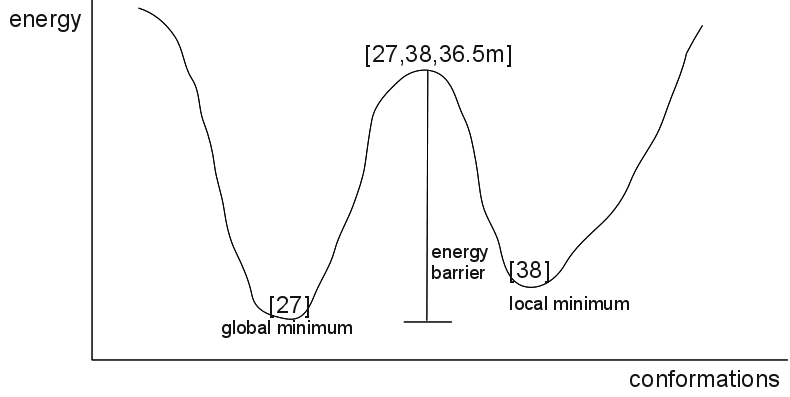
\includegraphics[scale=0.4]{images/energy_barrier.jpg} 
\end{figure}
\end{frame}

% frame 16
\begin{frame}
\frametitle{Possible problem}
  \scriptsize
  %Although the helices space grows considerably slower than structure space, but
  %it is still exponential

  %Growth of structure, helix and shape space
  Although both the abstract shapes and helices indices space grow exponentially with sequence length and suboptimal energy range, 
  the helices indices space grows considerably faster.
  \normalsize
  \begin{block}{\tiny comparison of helices indices space with abstract shapes space}
  %\begin{figure}
    \centering
	\begin{tikzpicture}[scale=0.7]
		%\begin{semilogyaxis}[xlabel=Index,ylabel=Value]
		%\addplot gnuplot[color=blue,mark=*]{1.2196*(x**(-1.5))*(2.6180**x)}; 
		%\end{semilogyaxis}
		\begin{semilogyaxis}[legend style={font=\small},xlabel={Sequence
         length},ylabel={Nr. of
         Structures/Helices/Shapes},width=\textwidth,legend style={nodes=right},
         legend pos= north west]
     
        
         %\addplot+[only marks,mark=+]
         %table[x=X,y=Y]{/home/jhuang/workspace/RNAHeliCes/scripts/estimate_exponent_RNAsubopt.txt};
         %\addlegendentry{Structures}         
         %\addplot table[x=X,y={create col/linear
         %regression={y=Y}}]{/home/jhuang/workspace/RNAHeliCes/scripts/estimate_exponent_RNAsubopt.txt};
         %\addlegendentry{$0.33 \cdot x -3.24$}
         
         
         \addplot+[only marks,mark=-]
         table[x=X,y=Y]{/home/jhuang/workspace/RNAHeliCes/scripts/estimate_exponent_RNAhelix.txt};
         \addlegendentry{Helices}         
         \addplot table[x=X,y={create col/linear
         regression={y=Y}}]{/home/jhuang/workspace/RNAHeliCes/scripts/estimate_exponent_RNAhelix.txt};
         \addlegendentry{$0.18 \cdot x -1.42$} 
 
         \addplot+[only marks,mark=x]
         table[x=X,y=Y]{/home/jhuang/workspace/RNAHeliCes/scripts/estimate_exponent_RNAshapes_5.txt};
         \addlegendentry{Shapes}                   
         \addplot table[x=X,y={create col/linear
         regression={y=Y}}]{/home/jhuang/workspace/RNAHeliCes/scripts/estimate_exponent_RNAshapes_5.txt};                 
         \addlegendentry{
$\pgfmathprintnumber{\pgfplotstableregressiona} \cdot x
\pgfmathprintnumber[print sign]{\pgfplotstableregressionb}$}
         
               
        
        %\addlegendentry{Legenden Eintrag};
        \end{semilogyaxis} 
	\end{tikzpicture}
	%\caption{Growth of structure, helix and shape space}	
  %\end{figure}	
  \end{block}
\end{frame}

% frame 17
\begin{frame}
\frametitle{Solution of possible problem}
  \small
  One of the solution: we limit the helices space by setting an energy range on
  it
  \normalsize
  \begin{block}{\tiny comparison of helices indices space setting different energy ranges}     
    \centering
	\begin{tikzpicture}[scale=0.7]
		%\begin{semilogyaxis}[xlabel=Index,ylabel=Value]
		%\addplot gnuplot[color=blue,mark=*]{1.2196*(x**(-1.5))*(2.6180**x)}; 
		%\end{semilogyaxis}
		\begin{semilogyaxis}[legend style={font=\tiny},xlabel={Sequence
         length},ylabel={Nr. of Helices},width=\textwidth,legend
         style={nodes=right}, legend pos= north west]

         \addplot+[only marks,mark=-]
         table[x=X,y=Y]{/home/jhuang/workspace/RNAHeliCes/scripts/estimate_exponent_RNAhelix.txt};
         \addlegendentry{energy range unlimited}
         \addplot table[x=X,y={create col/linear
         regression={y=Y}}]{/home/jhuang/workspace/RNAHeliCes/scripts/estimate_exponent_RNAhelix.txt};
         \addlegendentry{$0.18 \cdot x -1.42$} 

          \addplot+[only marks,mark=x]
          table[x=X,y=Y]{/home/jhuang/workspace/RNAHeliCes/scripts/estimate_exponent_RNAhelix_5_20kcal.txt};
          \addlegendentry{energy range 20kcal/mol}
          \addplot table[x=X,y={create col/linear
          regression={y=Y}}]{/home/jhuang/workspace/RNAHeliCes/scripts/estimate_exponent_RNAhelix_5_20kcal.txt}; 
          \addlegendentry{$0.12 \cdot x +0.44$} 
       
          \addplot+[only marks,mark=x]
          table[x=X,y=Y]{/home/jhuang/workspace/RNAHeliCes/scripts/estimate_exponent_RNAhelix_5_15kcal.txt};
          \addlegendentry{energy range 15kcal/mol}
          \addplot table[x=X,y={create col/linear
          regression={y=Y}}]{/home/jhuang/workspace/RNAHeliCes/scripts/estimate_exponent_RNAhelix_5_15kcal.txt};
          \addlegendentry{$0.0904 \cdot x +1.23$} 

          \addplot+[only marks,mark=x]
          table[x=X,y=Y]{/home/jhuang/workspace/RNAHeliCes/scripts/estimate_exponent_RNAhelix_5_10kcal.txt};
          \addlegendentry{energy range 10kcal/mol}
          \addplot table[x=X,y={create col/linear
          regression={y=Y}}]{/home/jhuang/workspace/RNAHeliCes/scripts/estimate_exponent_RNAhelix_5_10kcal.txt};
          \addlegendentry{$0.0602 \cdot x +1.43$}      
                                        
          \addplot+[only marks,mark=x]
          table[x=X,y=Y]{/home/jhuang/workspace/RNAHeliCes/scripts/estimate_exponent_RNAhelix_5_5kcal.txt};
          \addlegendentry{energy range 5kcal/mol}
          \addplot table[x=X,y={create col/linear
          regression={y=Y}}]{/home/jhuang/workspace/RNAHeliCes/scripts/estimate_exponent_RNAhelix_5_5kcal.txt};
          \addlegendentry{$0.0366 \cdot x +0.7$} 
     
                            
%           \addlegendentry{
%  $\pgfmathprintnumber{\pgfplotstableregressiona} \cdot x
%  \pgfmathprintnumber[print sign]{\pgfplotstableregressionb}$}
         
               
        
        %\addlegendentry{Legenden Eintrag};
        \end{semilogyaxis} 
	\end{tikzpicture}
  \end{block}	
\end{frame}


% PART 4: outlook   
% frame 18
\begin{frame}
\frametitle{Outlook: Designing RNA class predictors}
    \begin{itemize} 
    \item Development of a new structure abstraction (helices index)
    \item Implementation of an algorithm based on the structure abstraction
    \item Evaluating the algorithm
    \item Designing RNA class predictors.
    \end{itemize}
\end{frame}

% frame 19
\begin{frame}
\frametitle{End}
   \begin{itemize} 
   \item Thanks a lot for your attention !
   \item Questions ?
   \end{itemize}
\end{frame}


\end{document}
